\documentclass[../main.tex]{subfiles}
\graphicspath{{\subfix{../images/}}}
\begin{document}
\subsection{Terminology}
We start with a sampling of $\overrightarrow{Y}\sim f_{\theta}(\overrightarrow{y})$. We then get 2 \textbf{hypotheses} - $H_0$ (this is called the null hypothesis), and $H_1$ (alternative hypothesis). In theory these are interchangeable but, as the names suggest, traditionally $H_0$ is the "current thinking" or the one that is easier to check for and $H_1$ is the hypothesis that we want to check and compare. It is then widely said we "reject" or "accept" only about $H_1$. \\\\
What these hypotheses are in a sense are just the sets of coefficients that we find "usable" in our model. Formally
\[H_0 = \Theta_0\subset \Theta, \text{ } H_1 = \Theta_1\subset\Theta_1\text{ where } \Theta_1\cap\Theta_2=\emptyset\]
Hypotheses with one coefficient possible are called simple, and otherwise composite. 
\begin{definition}
A test statistic is a statistic where it gets "low" values for the null hypothesis, and "high" for the alternative hypothesis. 
\end{definition}
\begin{example}
If we take the birth sampling example the null hypothesis will naturally be that with equal probability females and males. And so it is natural to choose the following test statistic - 
\[T(\overrightarrow{Y}) = |\bar{Y}-0.5|\]
In this example it is then natural to choose $C>0$ such that if $T(\overrightarrow{Y})>C$ we accept $H_1$ and otherwise we reject the alternative hypothesis. This $C$ is called the critical value. If there isn't one emergent critical value for what we want it is accepted that you augment the statistic until there is a singular critical value.  
\end{example}
Now there is additional terminology
\begin{center}
    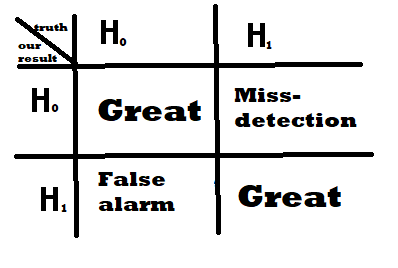
\includegraphics{images/Table For Stat Thoery.png}
\end{center}
Where miss-detection is an error of the second type, and false alarm is an error of the first type. The reason there is a distinction is again for real life reasons. We will assume for the lecture that both hypotheses are simple. We want to develop a strategy to choose which hypothesis is better. The probability to be wrong is the probability of having a type-1 error and the probability of having a type-2 error. These are
\[\mathbb{P}_{\theta_0}(T\geq C) \text{ for a type-1 error, } \mathbb{P}_{\theta_1}(T<C) \text{ for a type-2 error}\]
Now we denote
\[\Omega_0 := \{\overrightarrow{y}\mid T(\overrightarrow{y})<C\}\text{, }\Omega_1 := \{\overrightarrow{y}\mid T(\overrightarrow{y})\geq C\}\]
\begin{definition}
We define the significance of a test statistic to be the probability that we get an error of type 1 - 
\[\alpha:=\mathbb{P}_{\theta_0}(\text{"Accept "} H_1)=\mathbb{P}_{\theta_0}(\overrightarrow{Y}\in\Omega_1)\]
And we define $\beta$ to be
\[\beta:=\mathbb{P}_{\theta_1}(\text{"Reject "} H_1)=\mathbb{P}_{\theta_1}(\overrightarrow{Y}\in\Omega_0)\]
The power of the test is
\[\pi=1-\beta\]
\end{definition}
\newpage
\begin{example}
Assume there is a claim that a car gets 15 kilometers per liter, and the competition claims that their car gets 12 kilometers per liter. Let's assume a model where the sampling is $Y_i\sim\mathcal{N}(\mu, 4)$ where 
\[H_0:\mu=12,\text{ }H_1:\mu=15\]
Of course it makes sense to choose $\bar{Y}$ as the test statistic. If for example we have 5 samplings we have that
\[\bar{Y}\sim\mathcal{N}(\mu,\frac{4}{5})\]
We now want to calculate $\alpha$. If we for example take $C=14$
\[\alpha = \mathbb{P}_{\mu=12}(Y\geq 14) = 1-\Phi\left(\frac{14-12}{\sqrt{0.8}}\right) = 0.0127\]
And we have that
\[\beta = \mathbb{P}_{\mu = 15}(Y<C) = \Phi\left(\frac{14-15}{\sqrt{0.8}}\right) = 0.1318\]
This is all exemplified by the following image
\begin{center}
    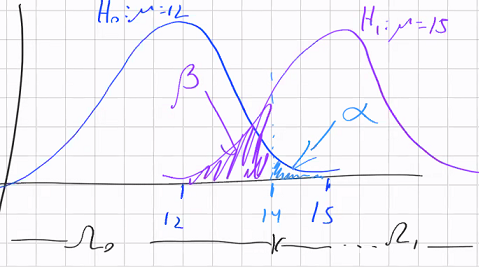
\includegraphics{images/Visualization For Stat Thoery.png}
\end{center}
\end{example}
\newpage
Now we can wonder what critical value is good. We can consider a few values for the critical value and see how it affects $\alpha$ and $\beta$. We can get the following table
\begin{center}
    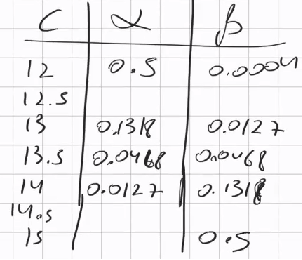
\includegraphics{images/Table 2 For Stat Thoery.png}
\end{center}
Regularly $\alpha$ is chosen arbitrarily at $0.05$.
\subsubsection{p-value}
Given a sampling $\overrightarrow{y}$ we can calculate 
\[t_{\text{obs}} = T(\overrightarrow{y})\]
\begin{definition}
The p-value of an experiment is
\[\text{p-value}:=\mathbb{P}_{H_0}\left(T(\overrightarrow{Y})\geq t_{\text{obs}}\right)\]
\end{definition}
And a lot of times it is demanded that the p-value be less than the previous threshold.  
\newpage
\subsection{Tests With Maximal Power}
For a given level of $\alpha$ it is natural to take a statistic that maximizes the power of the test, over all of the tests with a probability of error of type-1 $\leq\alpha$. 
\begin{definition}
Given a sampling $\overrightarrow{Y}\sim f_{\theta}(\overrightarrow{y})$, and 2 simple hypotheses
\[H_0:\theta = \theta_0\text{, }H_1:\theta=\theta_1\]
The likelihood ratio is 
\[\lambda(\overrightarrow{y}):=\frac{L(\theta_1;\overrightarrow{y})}{L(\theta_0; \overrightarrow{y})}\]
The likelihood ratio test (LRT), with significance $\alpha$ is if given a critical value of C we have that
\[\mathbb{P}_{\theta_0}(\lambda(\overrightarrow{y})\geq C)=\alpha\]
\end{definition}
\begin{lemma}[Neyman-Pearson]
Under these conditions LRT is a test with maximal power 
\end{lemma}
\begin{proof}
Will be shown next lecture. 
\end{proof}
\end{document}